

\emph{Vaadin}~\cite{vaadin} es un \textbf{framework} para el desarrollo de aplicaciones \emph{web} avanzadas, también conocidas como \emph{Rich-Internet Applications (RIA)}~\cite{ria}. El objetivo del paradigma \emph{RIA} es desarrollar aplicaciones \emph{web} con interfaces avanzadas que les haga asemejarse a las aplicaciones de escritorio. La principal ventaja que aporta \emph{Vaadin} es que permite escribir aplicaciones en código Java, como si fuesen de escritorio, y luego este código es transformado para que funcione en tecnologías web como HTML (HyperText Markup Language)~\cite{html}, CSS (Cascading Style Sheets)~\cite{css}, Javascript~\cite{javascript}, HTTP (Hypertext Transfer Protocol)~\cite{http} o AJAX (Asynchronous JavaScript and XML)~\cite{ajax}.

Una de las características diferenciadores de \texttt{Vaadin} es que, al contrario de las librerías de JavaScript tradicionales, \emph{Vaadin} también contempla la parte del servidor, por lo se generan tanto las llamadas al servidor desde la interfaz gráfica (\emph{front-end}) como la recepción y tratamiento de esas llamadas en la parte del servidor (\emph{back-end}).



 	
 \subsection{Ejemplo Vaadin}
 	
\begin{figure}[!tb]
	\centering
	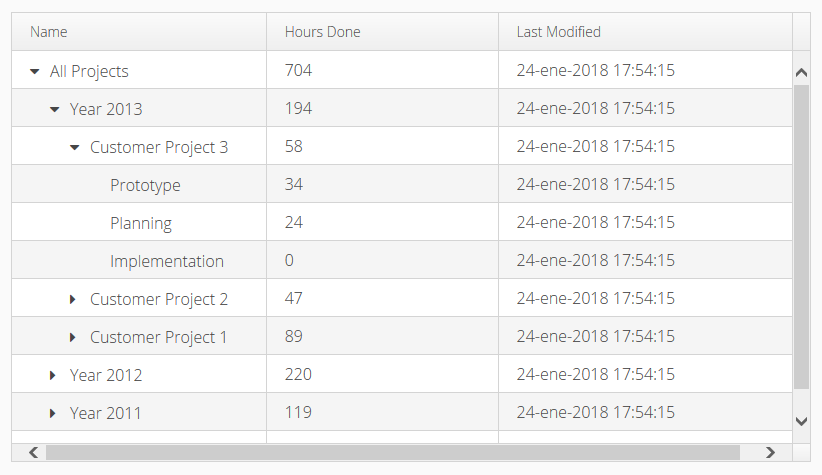
\includegraphics[width=\linewidth]{vaadinExampleImage.png}
	\caption{Árbol de Proyectos}
	\label{fig:vaadinExampleImage}
\end{figure}

A continuación, se explica un ejemplo de contrucción de una jerarquía de tareas propias en la gestión de proyectos por parte de un Jefe de Proyecto (Figura~\ref{fig:vaadinExampleImage}).

El proyecto creado para realizar el ejemplo se compone de una interfaz de usuario (Figura~\ref{fig:uiVaadin}) la cuál utiliza un componente llamado TreeGrid  (será explicado posteriormente,Figura~\ref{fig:treeGrid}) y un contenedor de datos (Figura~\ref{fig:demoContainer}).

Para entrar en contexto con la implementación de un proyecto en Vaadin, es necesario recalcar que el objetivo es abstraer al usuario de todo el comportamiento gráfinco implementado en HTML o Javascript, por lo tanto, para poder crear las estructuras que finalmente desembocarán en elementos gráficos, Vaadin utiliza los llamados componentes.

Un componente es una interfaz de alto nivel, todo elemento gráfico que se quiera utilizar debe de implementar y extender de las clases \emph{Component}\cite{componentVaadin} y \emph{AbstractComponent}\cite{abstractComponentVaadin}, estas constan de toda la implementación por defecto necesaria para poder mostrar un elemento.

La Figura~\ref{fig:uiVaadin} reprensenta la interfaz gráfica que se ha implementado para el ejemplo. En ella podemos ver que se ha creado un \emph{layout} o espacio reservado en la interfaz para insertar componentes, y se le han establecido dos características, la primera es un espaciado vertical y la segunda es un espaciado horizontal (Figura~\ref{fig:uiVaadin}, Líneas~4-6).

Posteriormente se declara el componente \emph{TreeGrid} que será el encargado de representar la jerarquía de elementos, además, se le ha dado un ancho y alto al elemento de 800 y 450 píxeles respectivamente (Figura~\ref{fig:uiVaadin}, Líneas~8-10).

Para que un componente muestre datos se le debe de insertar un contenedor de datos, en nuestro caso se ha creado una clase que se explicará más adelante que proporciona esta característica, y se le insertado a dicho componente (Figura~\ref{fig:uiVaadin}, Líneas~12-13).

Por último, se ha añadido el componente al \emph{layout} y este al contenido de la interfaz (Figura~\ref{fig:uiVaadin}, Líneas~15-16).

\begin{figure}[!tb]
	\centering
	\begin{lstlisting}[language=Java]
	@Override
	protected void init(VaadinRequest request) {
	
		final VerticalLayout layout = new VerticalLayout();
		layout.setSpacing(true);
		layout.setMargin(true);
		
		final TreeGrid grid = new TreeGrid();
		grid.setWidth(800, Unit.PIXELS);
		grid.setHeight(450, Unit.PIXELS);
		
		DemoContainer container = new DemoContainer();
		grid.setContainerDataSource(container);
		
		layout.addComponent(grid);
		setContent(layout);
	}
	\end{lstlisting}
	\caption{Interfaz de Usuario Vaadin}
	\label{fig:uiVaadin}
\end{figure}




\begin{figure}[!tb]
	\centering
	\begin{lstlisting}[language=Java]
	public class TreeGrid extends Grid {
		
		@Override
		public void setContainerDataSource(Container.Indexed container) {
			if (container != null) {
				if (!(container instanceof Container.Hierarchical)) {
					container = new IndexedContainerHierarchicalWrapper(container);
				}
				
				if (!(container instanceof Collapsible)) {
					container = new ContainerCollapsibleWrapper(container);
				}
			}
			super.setContainerDataSource(container);
		}
	}
	\end{lstlisting}
	\caption{Componente TreeGrid}
	\label{fig:treeGrid}
\end{figure}






\begin{figure}[!tb]
	\centering
	\begin{lstlisting}[language=Java]
	public class DemoContainer extends HierarchicalContainer implements Collapsible, Measurable {
	
		static final String PROPERTY_NAME = "Name";
		static final String PROPERTY_HOURS = "Hours done";
		static final String PROPERTY_MODIFIED = "Last modified";
		
		public DemoContainer() {
			addContainerProperty(PROPERTY_NAME, String.class, "");
			addContainerProperty(PROPERTY_HOURS, Integer.class, 0);
			addContainerProperty(PROPERTY_MODIFIED, Date.class, new Date());
			
			for (Object[] r : DataSource.getRoot()) {
				addItem(r);
			}
			
			setItemSorter(new DemoItemSorter());
		}
		
		private void setProperties(Item item, Object[] values) {
			item.getItemProperty(PROPERTY_NAME).setValue(values[0]);
			item.getItemProperty(PROPERTY_HOURS).setValue(values[1]);
			item.getItemProperty(PROPERTY_MODIFIED).setValue(values[2]);
		}
	}
	\end{lstlisting}
	\caption{Contenedor TreeGrid}
	\label{fig:demoContainer}
\end{figure}

